\chapter{Human Memory and Learning}
\label{chap:modeling_memory}

Humans learn so that they can get a better fit to the environment: understanding and learning allow for better perception. This Chapter provides an overview on different theories of human learning and memorization. 

\section{Learning and prediction}
Learning theory  advances by quantifying neurobiological \textbf{responses to stimuli} with different levels of probability/stimulus-features. Learning optimizes perception and behavior, with \textbf{surprise} (sometimes called \textit{prediction error}) being a long-considered key component because it is \textbf{a clue to what people know}. Surprise can be measured through different means: physiologically (e.g. pupil dilation), via brain data, and others.
But the S-R (Stimulus-Response) approach depends on more than what people know: it is mediated by low-level perception, accumulation of evidence, report biases, and response-initiation processes (noise). Therefore studying the observed responses to stimuli might not be the best way to understand what people learn.
Moreover, S-R also ignores the issue of whether people use learning to construct \textbf{expectations or predictions}. Computer models do not exhibit this problem, but humans do. Actually, there is no guarantee that our behaviour depends on predictions: it might be that no anticipatory prediction is done before the stimulus is presented; there is huge debate on this topic.
Studies of expectation probe the state of a cognitive system prior to stimulus presentation and independent of stimulus-guided responses. We can measure the expectation of a distribution using the Shannon Entropy. This is related to the surprise to a sample from the distribution. If the sample differs much from the expectation, then the surprise is higher (the subject is learning).

We can use surprise to understand if a person has learned something (surprise means he/she has picked up a distribution): we can observe surprise with respect to event transitions (Markov matrix). We can further observe if a person has just learned the marginal probabilities (how much an event is frequent) or also the conditional probabilities (how frequent an event is after a given other event).

\subsection{Cashdollar et al. (2016)}
They show how \textbf{learning produces predictions}, and \textbf{predictions impact processing}. In particular, they manipulate the randomness of an environment and observe, through MEG, how people behave. Image categories are presented \textbf{randomly} (\texttt{Rand}) or \textbf{predictably} (\texttt{Ord\_75}). Figure \ref{fig:cashdollar} shows that pre-stimulus activity is positively correlated with \textit{Working Memory Capacity} (WMC). \textit{Theta} and \textit{alpha} frequencies effects are observed to understand what happens in the brain. The strength (amplitude) of \textit{theta} oscillations gives a measure of how much the memory activity is involved.

\begin{figure}[!ht]
    \centering
    \captionsetup{width=.8\linewidth}
    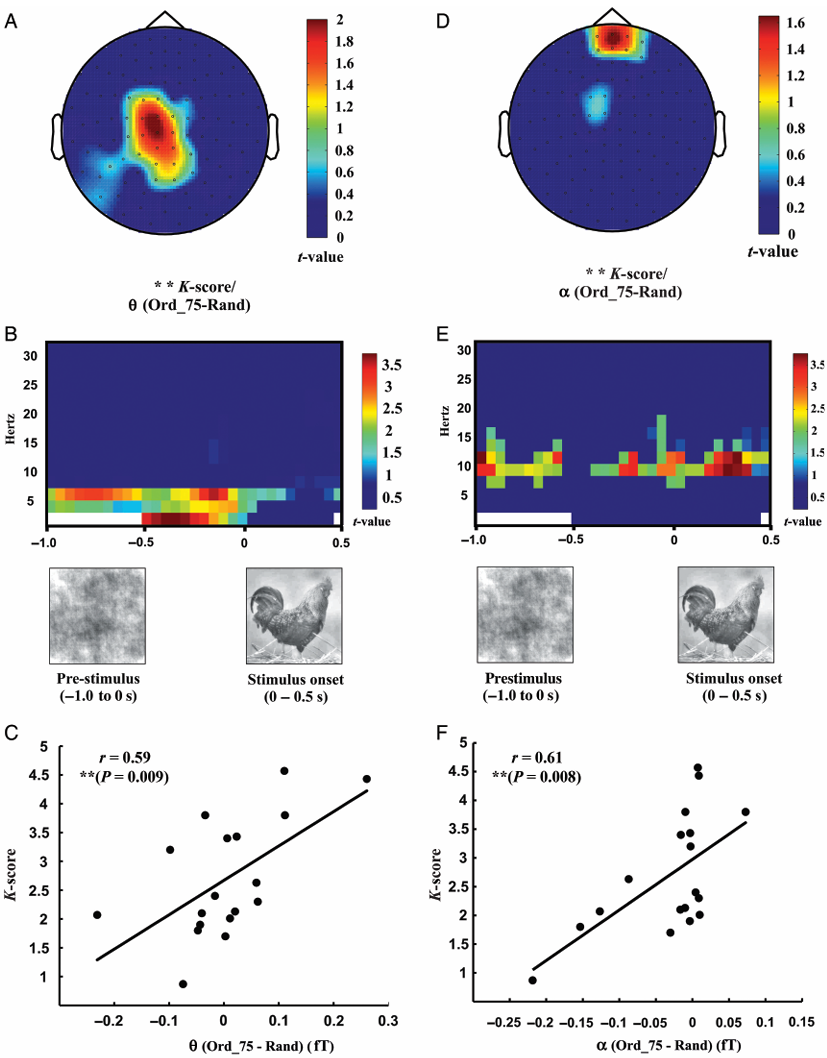
\includegraphics[width=0.75\linewidth]{images/cashdollar.png}
    \caption{Pre-stimulus oscillations and WMC (time 0 is when the next image is presented). Specifically, \textbf{(A)} pre-stimulus power differences in the $\theta$ band (4-8 Hz) between \texttt{Ord\_75} and \texttt{Rand} trials positively correlate with individuals' K-scores within a cluster of central sensors \textbf{(C)} and continue throughout the entire pre-stimulus period but terminates with the onset of the stimulus \textbf{(B)}. Similarly, within a cluster of frontal sensors \textbf{(D)} pre-stimulus power differences in the $\alpha$ band (8–12 Hz) between \texttt{Ord\_75} and \texttt{Rand} trials also positively correlate with individual's K-scores \textbf{(F)}, yet this pattern continues throughout stimulus presentation \textbf{(E)}.}
    \label{fig:cashdollar}
\end{figure}

They also measure how pre-stimulus activity (as a function of regularity \notet) relates to post-stimulus activity. They observe  stronger activity for predictable stimulus ($\text{\texttt{Ord\_75}}-\text{\texttt{Rand}}$, Fig. \ref{fig:cashdollar_2}) for people more sensitive to series order (greater pre-stimulus $\theta$ band power for ordered~vs.~random series). In other words, people who make predictions (those who have learned the distributions, i.e., that have higher post-stimulus activity) are also those having higher pre-stimulus activity.

\osst{As a function of regularity because they manipulate the degree of predictability (i.e., regularity) of the environment.}

\begin{figure}[!ht]
    \centering
    \captionsetup{width=.8\linewidth}
    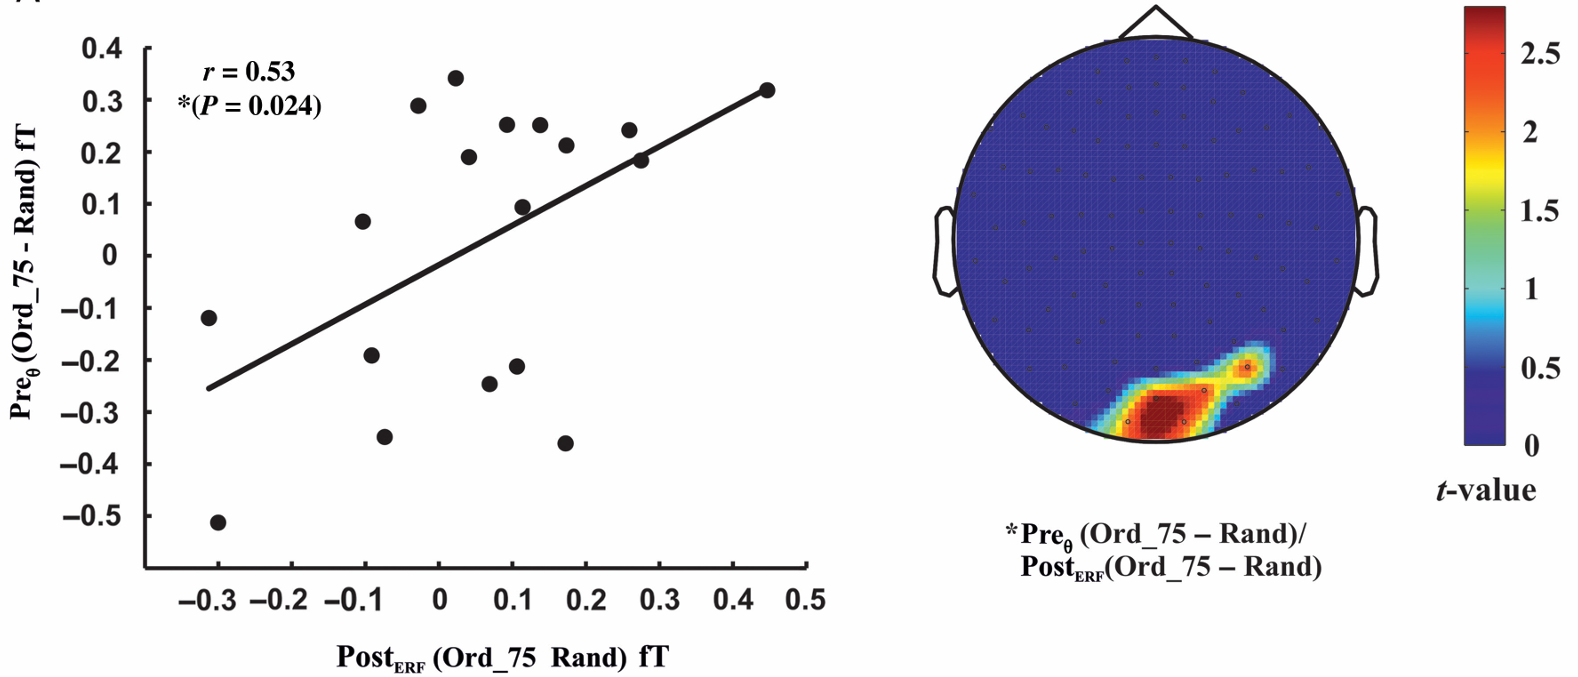
\includegraphics[width=0.7\linewidth]{images/cashdollar_2.png}
    \caption{Pre-stimulus oscillations and post-stimulus neural responses. For each participant, they identified the sensor with the largest absolute pre-stimulus power difference ($\text{\texttt{Ord\_75}}-\text{\texttt{Rand}}$), within the $\theta$ (Pre$_\theta$) and $\alpha$ (Pre$_\alpha$) frequency bands separately (-1.0 to 0 s prior to stimulus onset).}
    \label{fig:cashdollar_2}
\end{figure}

\subsection{The logic of studying learning and prediction}
We need to quantify learning from observable behavior, to separate predictive processes from responses, and to quantify the relation between the two. To this end, in the following we consider \cite{notaro}, a study showing how \textbf{anticipatory fixation offsets carry more information about environmental statistics than reactive stimulus-responses}.

\section[Predictions as a window into learning]{\textit{Predictions as a window into learning}\\ \mandatory{notaro}}
They experiment with 21 volunteers. The person is looking at a screen (in the center). A target symbol is be presented on the right or on the left side of the screen. A Markov process determines the probability of the next target to be on the same side of the previous. If the probability is 70\% we call this \texttt{pret70}, if it is 30\% then \texttt{pret30} (``pret" stands for ``probability of return"). So in \texttt{pret70} the person (if they learn the pattern) should expect the next target to stay on the same side; while in \texttt{pret30} should expect it to change side.

\begin{figure}[!ht]
    \centering
    \captionsetup{width=.8\linewidth}
    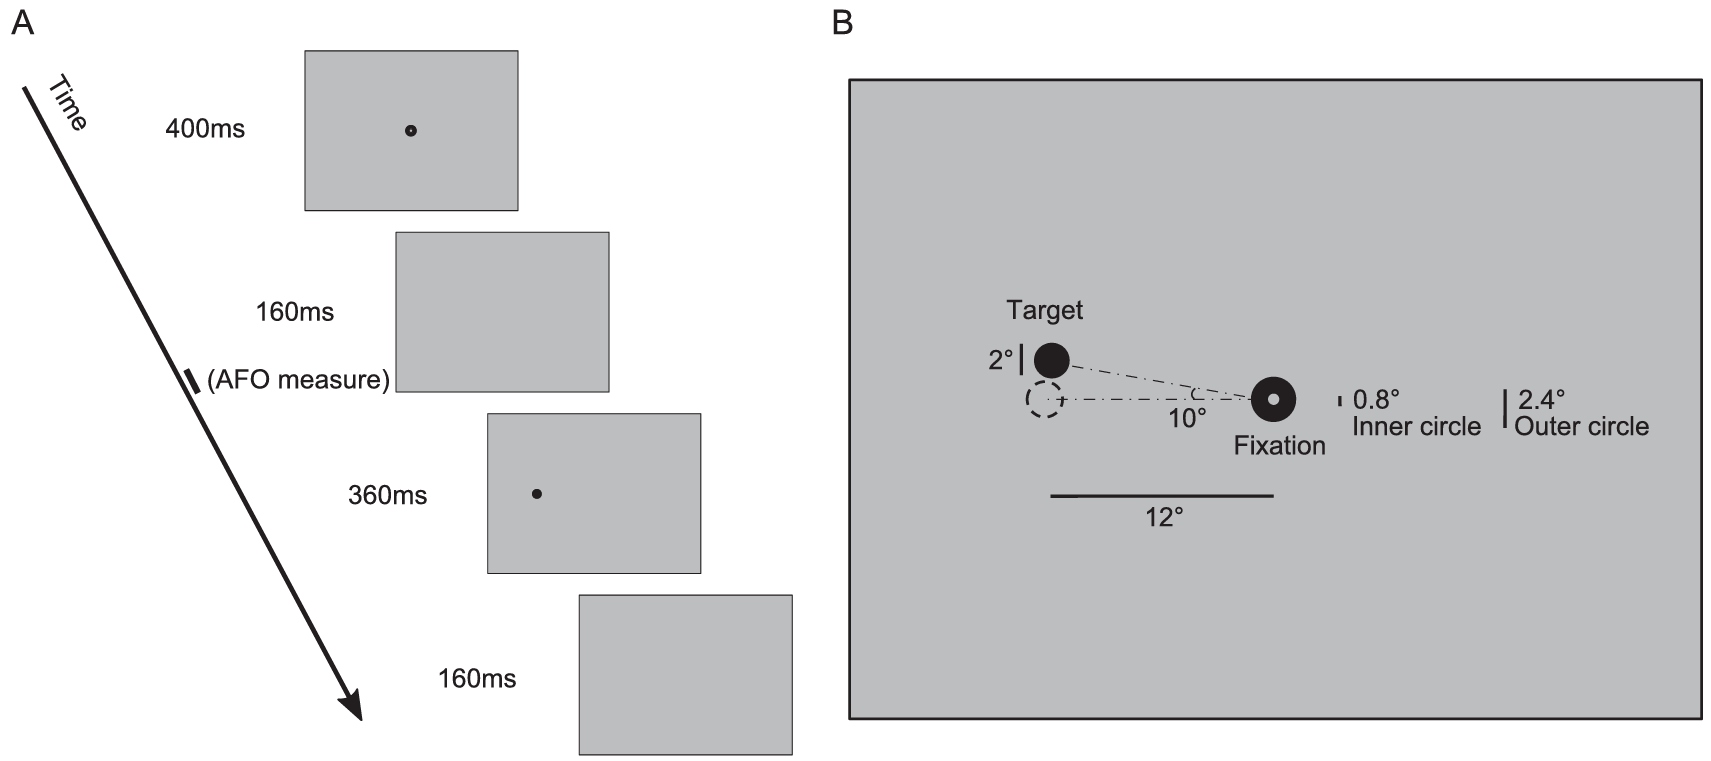
\includegraphics[width=0.7\linewidth]{images/notaro.png}
    \caption{Trial structure and fixation locations. \textbf{(A)} Trial timing: fixation symbol; blank screen; target; blank screen. This is repeated 100 times in a series. \textbf{(B)} Spatial features of fixation and targets. Targets are positioned on an invisible arc that extended 108 above and below the fixation symbol, at 128 eccentricity. The exact location on the arc is randomly set on each trial. The fixation symbol consists of an inner gray circle ($\text{radius} = 0.4\degree$) within an outer black circle ($\text{radius} = 1.2\degree)$.}
    \label{fig:notaro}
\end{figure}

\begin{wrapfigure}[17]{r}{0pt}
  \centering
  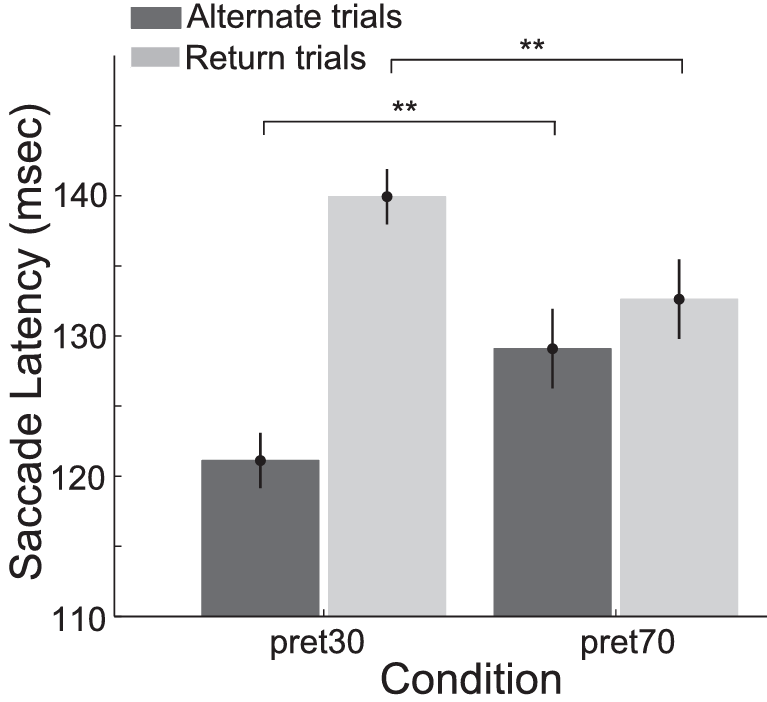
\includegraphics[width=0.3\textwidth]{images/saccade.png}
  \caption{Saccade latencies indicate learning of statistical structure in addition to an effect of whether a saccade is a return or alternation. Asterisks above bar pairs indicate significant difference.}
  \label{fig:saccade}
\end{wrapfigure}

10 series are presented in each condition, each one consisting in 100 trials (Figure \ref{fig:notaro}A shows what a single trial looks like).
The proportion of presentations on the left and right screen sides is 50\% in both conditions (the marginal probability is the same).
Moreover, 20 random-location trials are appended to each series to study wash-out effects. They use an eye-tracking system at 1000 Hz to capture the gaze.
They name ``Return trials" those for which the screen-side of the last-presented target is the same as the preceding one, and ``Alternation trial" for opposite side.

\subsection{Saccade latency}
The \textbf{saccade latency} is defined as the time taken from the appearance of a target to the beginning of a saccade (i.e., a rapid movement of the eye between fixation points) in response to that target. Note that the first 80 ms are ``consumed" by the signal travelling from eyes to the brain. Saccade latency can be used as a \textbf{measure of surprise}, and \textbf{provide evidence for learning}.

The results (Fig. \ref{fig:saccade}) show that saccades to target presented on alternate sides are faster when alternates are more predictable (\texttt{pret30}). Saccades to targets presented on return sides faster when returns are more predictable (pret70). In \texttt{pret30} subjects should expect an alternation, and indeed the results agree. However, in \texttt{pret70}, we do not have the opposite: in general, returns are slower than alternations because. This is because people do not like to return their attention where they already looked at: people like to explore and shift attention to any other place. This phenomenon has been named ``\textbf{inhibition of return}" (IOR).

\subsection{Anticipatory fixation offset}
They also investigate how people look at the fixation symbol while waiting for the next target.
They define the \textit{anticipatory gaze offset} as the absolute gaze location in relation to the center.

\begin{figure}[!ht]
    \centering
    \captionsetup{width=.8\linewidth}
    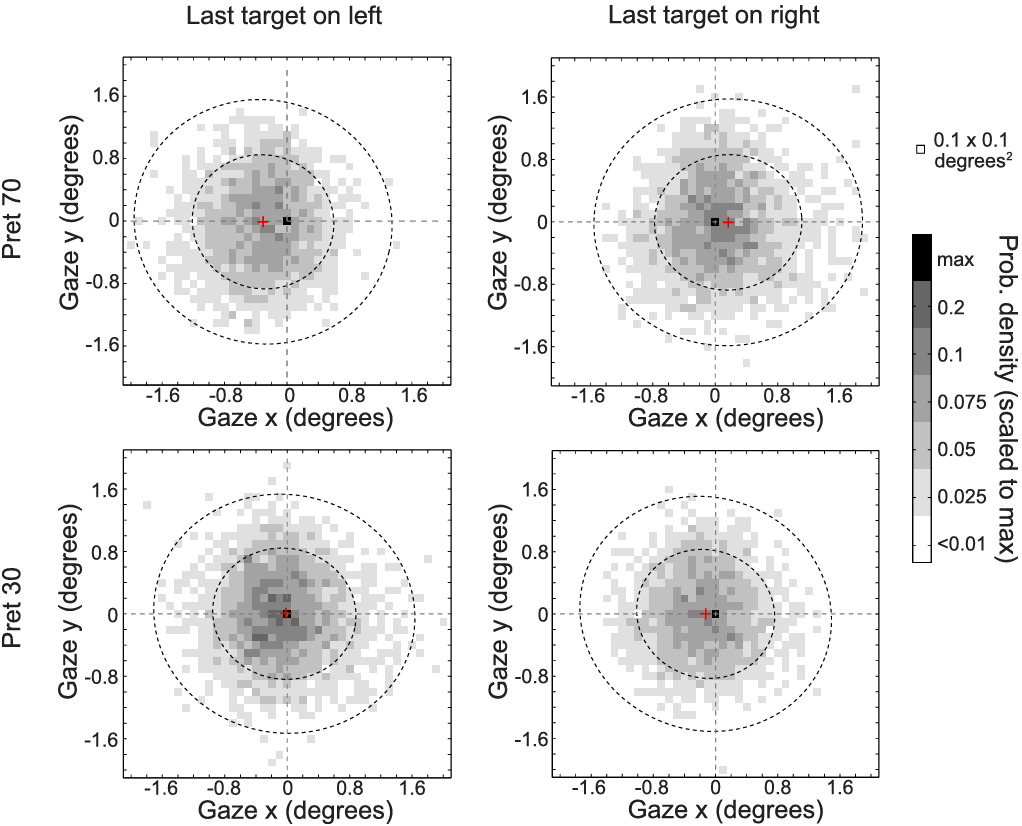
\includegraphics[width=0.6\linewidth]{images/afo.png}
    \caption{Density of fixation location during the last 10 ms of pre-target blank screen. The single dark point: screen center. Red points: mean values for condition; inner/outer circles mark areas encompassing 50\% and 90\% of all fixations. When returns are expected, anticipatory bias towards location of last target is observed.}
    \label{fig:afo}
\end{figure}

The \textbf{\textit{anticipatory fixation offset}} (\textbf{AFO}) is the recording of the gaze offset in relation to the prior target: horizontal deviation from the center is coded as positive if to the side of the last presented target, negative otherwise. The AFO is measured during the final 10 ms of pre-target blank screen. It is arbitrarily coded as positive for offsets to the side of the last presented target. This is a \textbf{measure of anticipatory behaviour} (i.e., ``how much people are betting that the target will appear on a specific side, instead of the other"). If an individual does not learn the environment, the average AFO is expected to be 0.

\begin{figure}[!ht]
    \centering
    \captionsetup{width=.8\linewidth}
    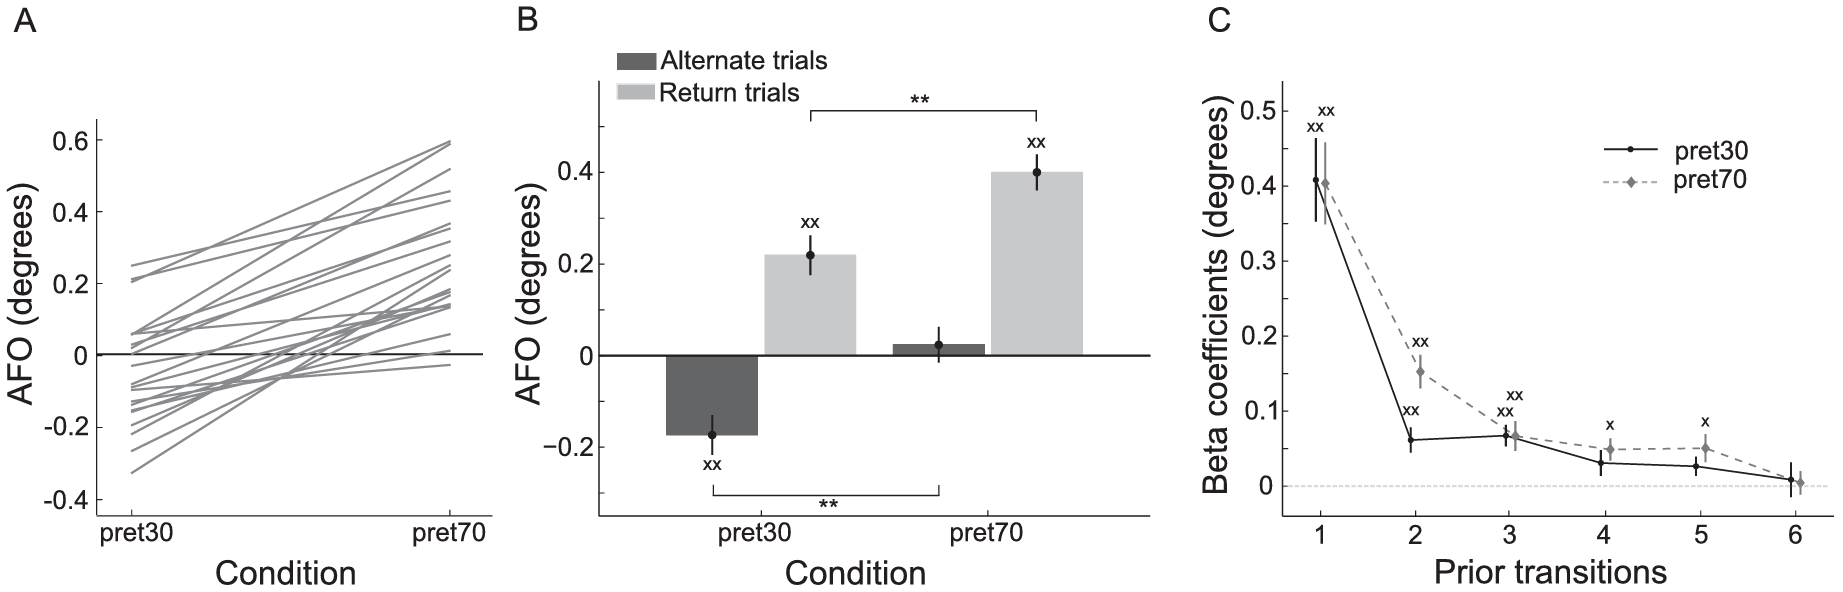
\includegraphics[width=0.9\linewidth]{images/afo_2.png}
    \caption{The impact of statistical structure on AFO. \textbf{(A)} Mean AFO values were significantly greater in \texttt{pret70} than \texttt{pret30}, and the pattern held for all participants (each participant marked via single line). Notice for \texttt{pret30} the mean AFO is negative for some participants. \textbf{(B)} Partitioning AFO values by most recent transition indicates an effect of statistical structure as well as an impact of most recent transition, as AFO was greater following returns than following alternate trials. \textbf{(C)} Beta weights estimated via regression models indicate that AFO was impacted by a return in each of the last five transitions in the \texttt{pret70} condition and in each of the last three transitions for \texttt{pret30}.}
    \label{fig:afo_2}
\end{figure}

They observe that \textbf{AFO indicates active prediction}. Consider the results in Fig. \ref{fig:afo_2}B; in \texttt{pret70}, ideally (to maximize probability), people should bet on return every time, however this is not the case: they strongly bet on return if the last trial was a return, while the average AFO is almost 0 if the last trial was an alternation. In \texttt{pret30} they should always bet on alternation, however they strongly bet on return if the last trial was a return. This demonstrates the \textbf{independent impact of the very last trial}, which might be caused by the fact that human environments are typically non stationary (meaning that they change distribution over time), so people are used to continuously learn (\textit{explore} instead of \textit{exploit knowledge}). Nevertheless, the behavior is subtle: AFO values $\sim 0.4\degree$ from the center (12 pixels on a Full HD screen, a small yet significant shift).\\

To validate the results, they use \textbf{split-half} (SH) \textbf{reliability}. The statistic used is the AFO difference between \texttt{pret30} and \texttt{pret70} ($\Delta AFO = AFO_{\text{\texttt{pret70}}} - AFO_{\text{\texttt{pret30}}}$), computed for each single participant. They derive two separate $\Delta AFO$ values per participant: one from odd trials and one from even trials. Using rank order correlation, they find a SH correlation of 0.9, which proves the reliability of this study.

\subsection{Time scale of learning}
Even when there is predictable regularity in the world, people do not always predict the most likely outcome (we saw: strong impact of last trial, people are not ``ideal Bayesian observers", i.e., they do not allocate the same importance/weight to all past events). This is irrational: people would be most successful if they always bet on the most likely outcome. Still, people cannot ignore the impact of the most recent past (perhaps useful for non-stationary environments). For this reason there is a need for a Mathematical Modeling approach to quantify how information is integrated over time to determine the current behavior. The model can be applied to quantify responses (saccade latency) or prediction (AFO). Such mathematical approach also allows them to reverse engineer the predictions (to look at the past events that have been allocated more weight).

They use a simple linear regression to model the impact of 6 prior transitions:
\[
AFO = \beta_1S_1 + \beta_2S_2 + \beta_3S_3 + \beta_4S_4+ \beta_5S_5+ \beta_6S_6 + c + \epsilon
\]
Where $S=1$ if the last target is a return and $S=0$ if the last target is an alternation; $\beta_k$ are weights to be learned.  The regression model is fit per participant per condition (\texttt{pret70}, \texttt{pret30}).

Fig. \ref{fig:afo_2}C shows how the recent past impacts prediction. Recent return trials present a bias prediction towards the side of the most recent target, with a very strong effect of the last trial. The decay is rapid, even more for \texttt{pret30}; this has a lot of alternations, which lead humans to think there is less information to learn (it seems random) so they integrate over less trials.\\

They also model the saccade latency, instead of the anticipatory gaze. The regression model is fit per participant per condition, but separately for return and alternation saccades (control: IOR, surprise). The results show \textbf{no impact of recent past on response times for predicted targets} (alternation saccades in pret30, return saccades in \texttt{pret70}). Return saccades in \texttt{pret30} (surprising targets) present an impact limited to the immediately preceding transition: return saccades are faster when preceded by a return. For alternation saccades in pret70 the last 4 $\beta_k$ have significant impact: recent return trials slow down an alternation saccade (vs.~returns).\\

Saccade latencies confirm statistical learning, while AFOs reflct learning of global statistics. Saccade latencies reflect IOR, while AFOs do not. 
These findings show how modelling response to stimuli with respect to past events can give completely different results, as the past affects the two computational models in completely different ways, as preparatory process and actual execution of saccade are differently impacted.

\subsection{Time scales of knowledge consolidation and process of forgetting}

\begin{figure}[!ht]
    \centering
    \captionsetup{width=.8\linewidth}
    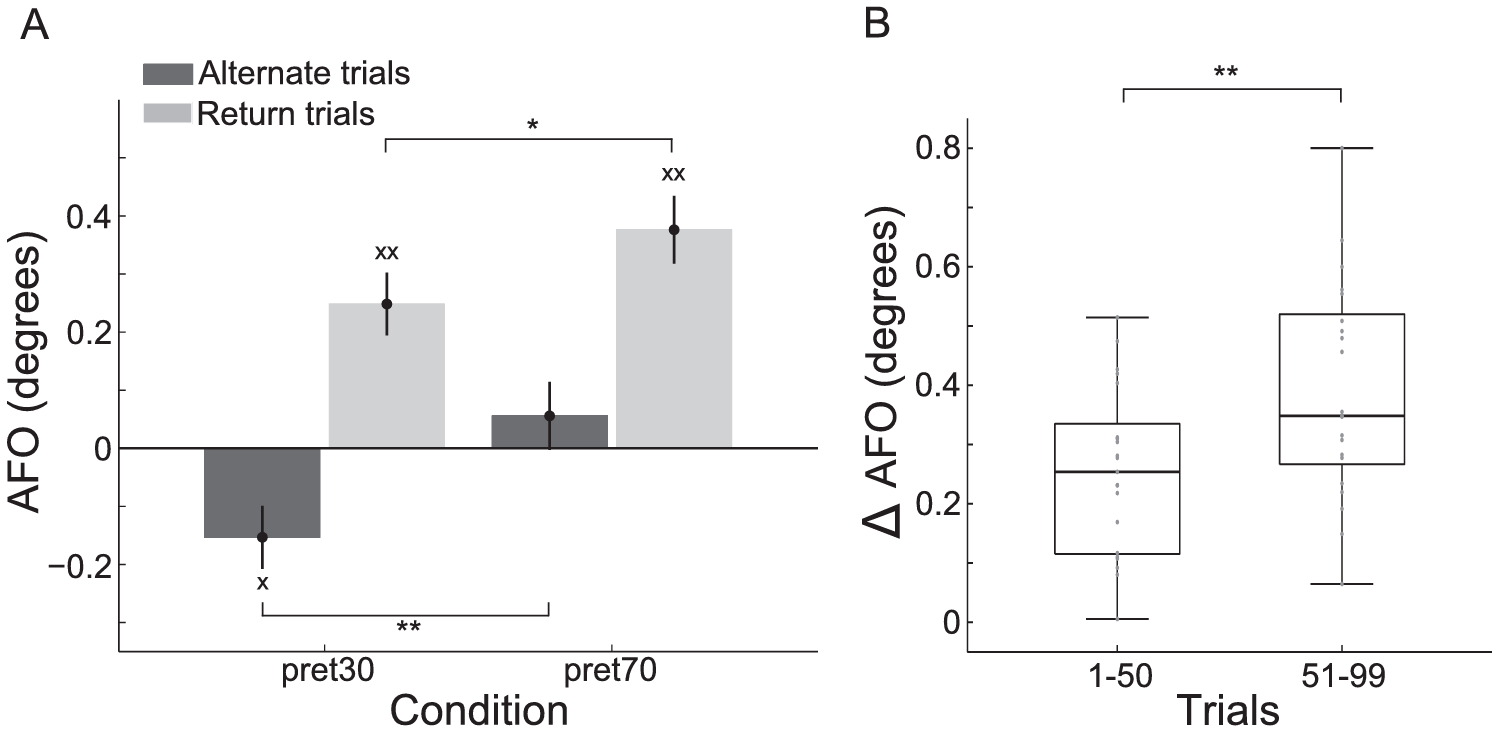
\includegraphics[width=0.55\linewidth]{images/afo_3.png}
    \caption{Long-term learning signatures in AFO. \textbf{(A)} AFO values in the 20 random trials (\texttt{pret} = 50\%) appended to each experimental series. Average AFO magnitudes indicate confinement to the area of the fixation symbol ($<0.4\degree$ eccentricity). There is a strong impact of the statistical structure of the series presented prior to the random trials, and independently, a strong impact of the immediately preceding trial. \textbf{(B)} $\Delta$AFO values significantly increased from the first half to the second half of the experimental series.}
    \label{fig:afo_3}
\end{figure}

They proceed by studying consolidation and forgetting on large timescales, questioning whether there is consolidation of knowledge over the entire set of 100 trials, and whether there is rapid forgetting during the washout trials (i.e., \texttt{pret50}, random trials). In Fig. \ref{fig:afo_3}B is noticeable how AFO increases over trials.
Moreover, previous statistics impact AFO during during washout: when forgetting, people still show effects of the prior statistical condition, and the immediately prior trial (consider Fig. \ref{fig:afo_3}A and compare it to Fig. \ref{fig:afo_2}B).

\subsection{Rescorla-Wagner learning model based on AFO}
They use an error-driven (Rescorla-Wagner) \textbf{model of learning} to map beliefs about transitions to observed behavior (AFO). They use it for predicting the actual human behaviour. The model is implemented as:
\[
\begin{cases}
    P_{ret}(t+1) = P_{ret}(t) + \alpha(1-P_{ret}(t)) \quad \text{after a return}\\
    P_{ret}(t+1) = P_{ret}(t) - \alpha P_{ret}(t) \quad \quad \quad \;\; \text{after an alternation}\\
    AFO(t+1) = K(P_{ret}(t+1)-P_0)
\end{cases}
\]
where $P_0$ is the probability equilibrium point \notet; $K$ is the scaling factor transforming internal probability to overt behavior; and $\alpha$ is the learning rate (the relative importance of a new observation in relation to prior knowledge). Note: both are learned for single individuals. $K$ links the internal belief (the probability) to the actual behaviour (AFO). Different people behave differently with the same internal belief, meaning that this parameter is not the same for everyone. Similarly, different people have very divergent learning rates.

The advantage of an error-driven learning model is that it allows to model the learning rate. This is directly related to the drop-off curve of the $\beta_k$ in the regression model (impact of past on present). The scaling factor $K$ further deals with the possibility that in different situations, the exact same knowledge can translate to behaviors of different magnitude; it can be seen as a measure of confidence.

\boxc{\notet Probability equilibrium point}{
    \textbf{People mis-estimate chance in a systematic way}: random binary series are subjectively perceived as containing too many streaks. In particular, people perceive the series as random when the probability of return is $\sim0.4$ (probability of alternation 0.6). On the other hand, if the probability is 0.5 they think there are too many returns. As a result, people do not start predicting returns when $P(ret)>0.5$. Their point of equilibrium is thought to be around $P(ret)=0.4$ instead.
}

They observe a huge variability among individuals (very different $\alpha$ and $K$). From a statistical perspective, \texttt{pret30} is as much informative as \texttt{pret70}, however people present higher learning rate in \texttt{pret30}. This because people would perceive \texttt{pret40} as random, not \texttt{pret50}; so psychologically \texttt{pret70} is considered to be much more informative than \texttt{pret30}.
They successfully validate on left-out data per participant.

\begin{figure}[!ht]
    \centering
    \captionsetup{width=.8\linewidth}
    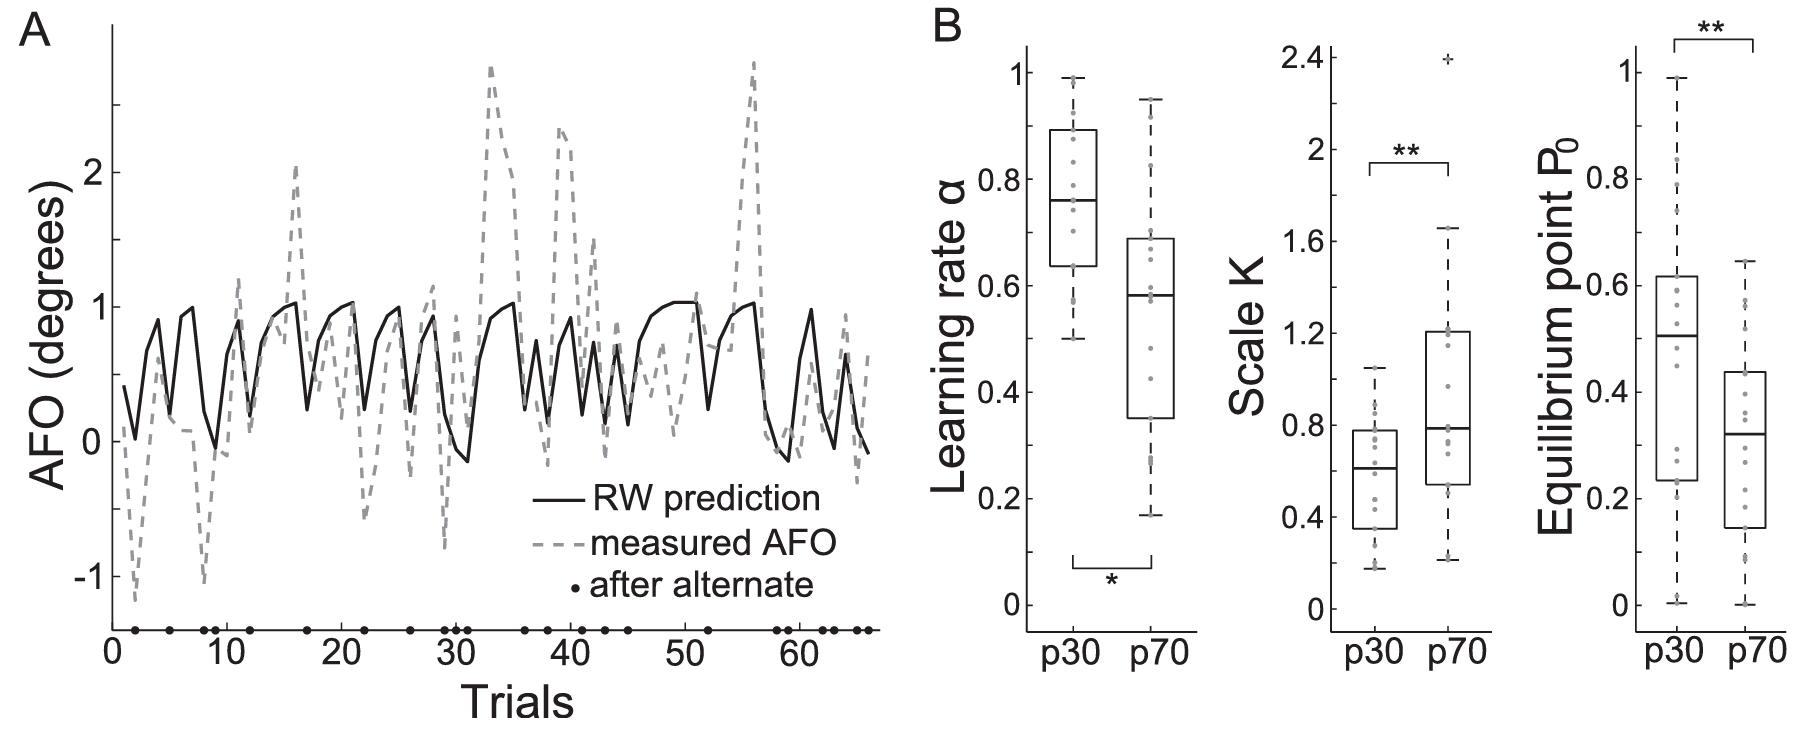
\includegraphics[width=0.75\linewidth]{images/rescorla.png}
    \caption*{Rescorla-Wagner model of AFOs. \textbf{(A)} AFO data from a sample series in \texttt{pret70} condition (dashed line) and the matched model prediction (continuous line) that was derived from parameter values estimated from independent series. Asterisks on abscissa mark alternate (side-switch) trials. Data are concatenated to exclude missing or invalid values. \textbf{(B)} Distributions of model parameters in the two conditions. From the left: learning rate, scaling factor, and equilibrium point. P0. The equilibrium point significantly departed from 0.5 only in \texttt{pret70}.}
    \label{fig:rescorla}
\end{figure}

In conclusion, the different learning rates for two processes with identical conditional entropy supports the idea of a subjective perception of randomness. Modulations of $K$ are consistent with greater confidence in executing behavior in \texttt{pret70}.

\section[Relationship between prediction and behavior]{Relationship between prediction and behavior\\ Timme and Lapish (2018)
}
They study the relationship between anticipation (anticipatory fixation offset, AFO) and stimulus response (saccade latency, SL), to understand if AFOs predict subsequent SLs in a manner consistent with prior prediction. They further want to know if there is a difference in the amount of information AFOs and SLs carry about the experimental condition, i.e., if it is possible to predict the condition (\texttt{pret30} or \texttt{pret70}) based on human behaviour.\\

If AFO measures prediction, the following relation should hold between measured AFO and following SL: larger AFO values (putative anticipation of target on prior side) should be followed by faster return saccades, but slower alternation saccades (negative AFO/SL correlation for returns, positive AFO/SL correlation for alternations). This is what is found. A larger anticipatory bias towards return predicts a faster return saccade, and also predicts a slower alternation saccade.\\

To answer the second question, they study which measure, AFO or SL, carries more information about the condition. They use \textbf{Mutual Information} (MI), as this captures the amount of knowledge one variable provides about another without assuming any particular relationship between the two variables (Fig. \ref{fig:timme}). Mutual information is expressed as:
\[
I(X;W) = H(X) - H(X|W) = \sum_{x \in X, w \in W} p(x,w) log_2 \left( \frac{p(x,w)}{p(x)p(w)} \right)
\]
where $X$ is the experimental condition; and $W=1,2\text{ or }3$ (respectively SL, SL$\vert$trial-type, and AFO).

\begin{figure}[!ht]
    \centering
    \captionsetup{width=.8\linewidth}
    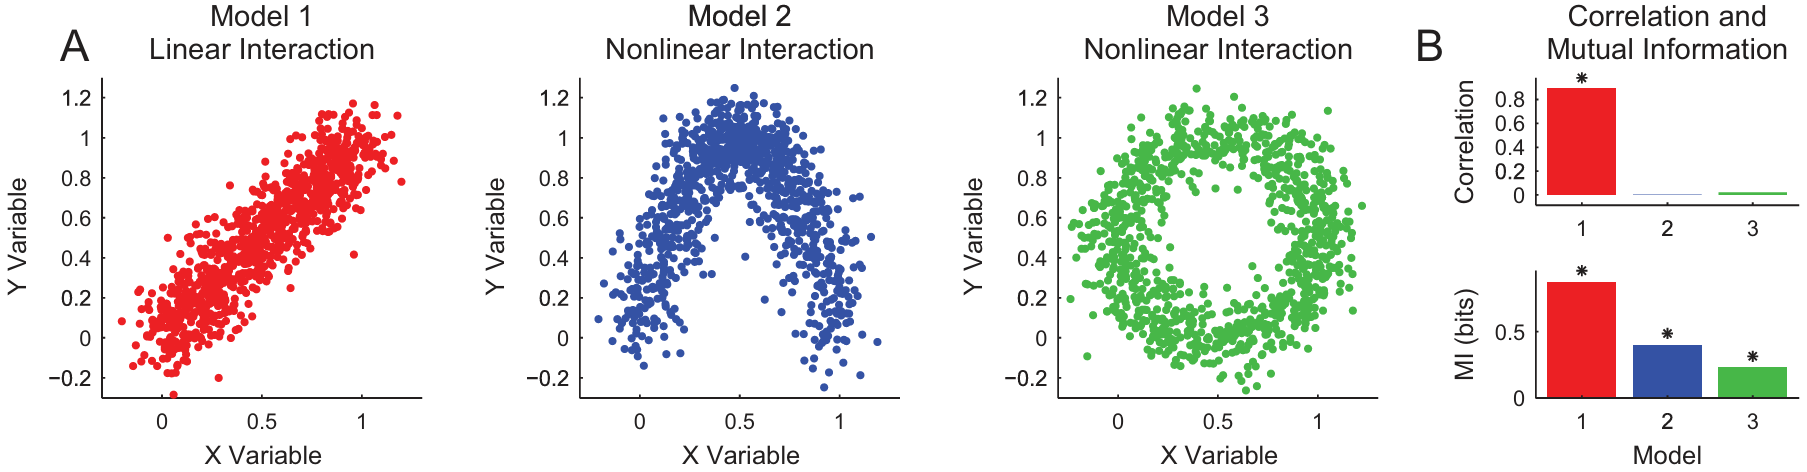
\includegraphics[width=0.85\linewidth]{images/timme.png}
    \caption{Example of linear versus nonlinear analysis methods. \textbf{(A)} Example data for three models (red, blue, and green) with linear (red) and nonlinear (blue and green) interactions; \textbf{(B)} the associated correlation coefficient and mutual information (MI) values for all three models.}
    \label{fig:timme}
\end{figure}

They find that AFO discriminates the 2 conditions (\texttt{pret70} and \texttt{pret30}) better than SL, conveying around twice as much information about the statistical process.
However, the amount of mutual information is quite low for both: $0.0527 \pm 0.0063$ vs. $0.0245 \pm 0.0050$. In general, AFOs contain more information about statistical context than that contained in SL distribution or SL distribution conditioned on trial-type.\\

To summarize what we have seen so far in this Chapter:
\begin{itemize}
    \item \textbf{Learning can be studied by quantifying observable behavior} over time;
    \item Macro-scale properties of the environment such as association-strength can be separated from micro-scale occurrences in recent past. Both impact behavior;
    \item \textbf{Learning translates into surprise signals}: people react more slowly to surprising events;
    \item \textbf{Learning produces anticipation/prediction}, which can be modeled with error-driven learning;
    \item Anticipatory signals can contain more information about the environment than stimulus-related responses.
\end{itemize}

\section{Human memory}
In the following is an overview of the history of learning and 
memory, with different theories and studies on human memory.\\

Psychological theories can be specialized to address questions on a variety of related levels of explanation, which can sometimes inform other levels, through a process called \textit{reductionism}:
\begin{itemize}
    \item Social-Psychological level: Awareness
    \item Cognitive level: Processes
    \item Physiological level: Neurons
    \item Biochemical level: Molecules
    \item Physical level: Atoms
\end{itemize}

\subsection{History of learning and memory}
\begin{figure}[!ht]
    \centering
    \captionsetup{width=.8\linewidth}
    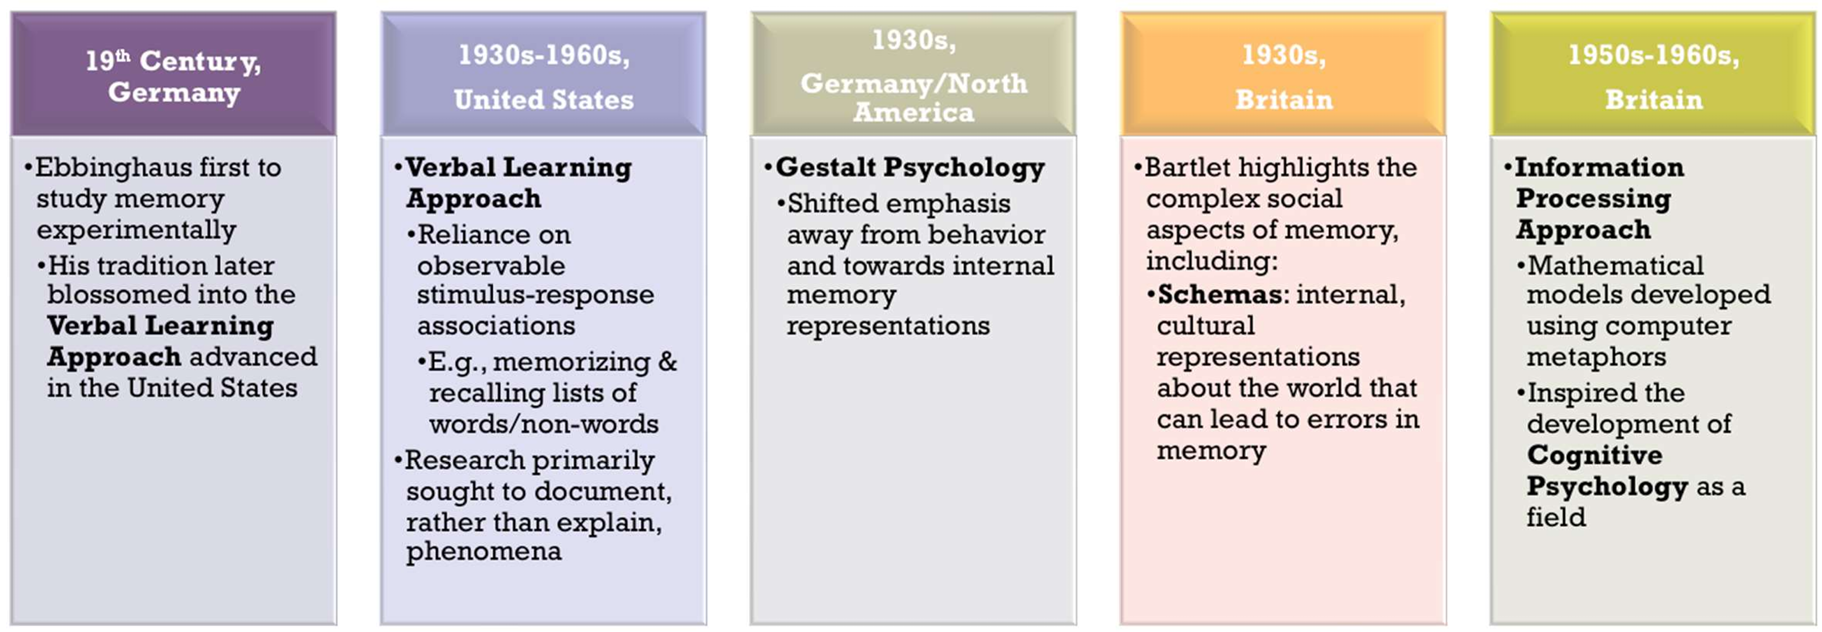
\includegraphics[width=0.9\linewidth]{images/memory.png}
    \caption*{Schematized history of learning and memory. Notice that the 3 theories in the middle were concurrent.}
    \label{fig:memory}
\end{figure}

\subsection{Ebbinghaus}

\begin{wrapfigure}[12]{r}{0pt}
  \centering
  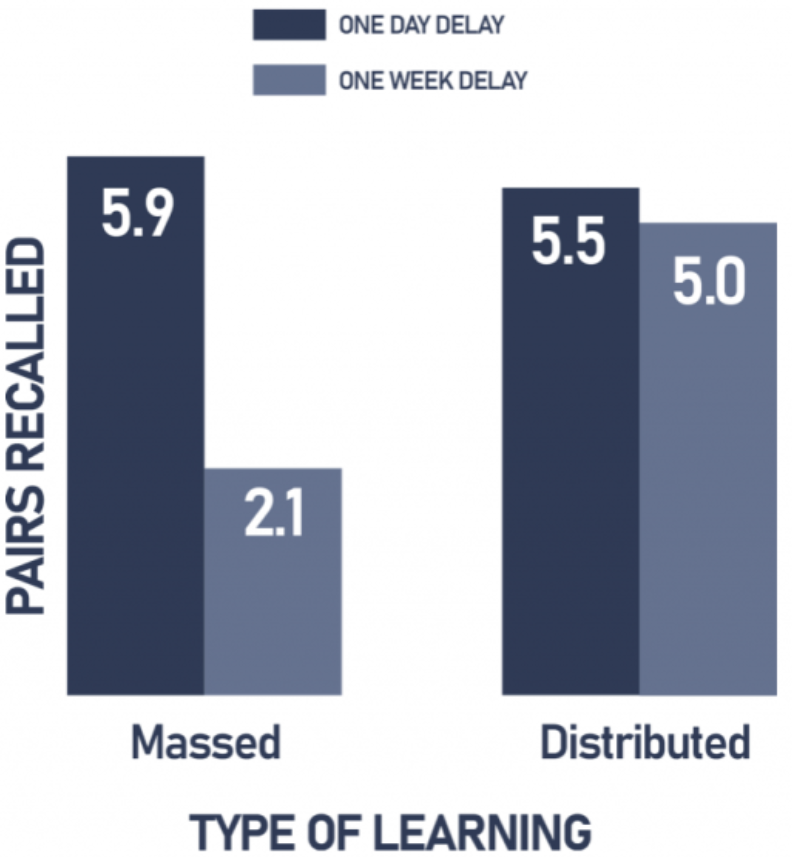
\includegraphics[width=0.25\textwidth]{images/keppel.png}
  \caption{Keppel (1967).}
  \label{fig:keppel}
\end{wrapfigure}

Ebbinghaus thought memory is a sort of storage.
He conducted an experiment in which people are presented some items. Almost all are items are memorized (immediate recall nearly 100\%). After 20 minutes, there is already a huge drop in information retention. However, not all information is lost, even after 31 days (Fig. \ref{fig:ebbinghaus}). He also found that the more repetitions (practice), the more likely 
information is to be remembered later (Fig.~\ref{fig:ebbinghaus_2}).
He used a list of nonsense syllables (as items) in order to have a cultural-independent study.\\
Ebbinghaus introduced another study: how memorization is impacted by the information composition.
Fig. \ref{fig:keppel} shows the difference between all items together (massed learning) vs.~a small chunck at a time (distributed learning).

\begin{figure}[!ht]
    \centering
    \captionsetup{width=.8\linewidth}
    \begin{subfigure}{.49\textwidth}
        \centering
        \captionsetup{width=.8\linewidth}
        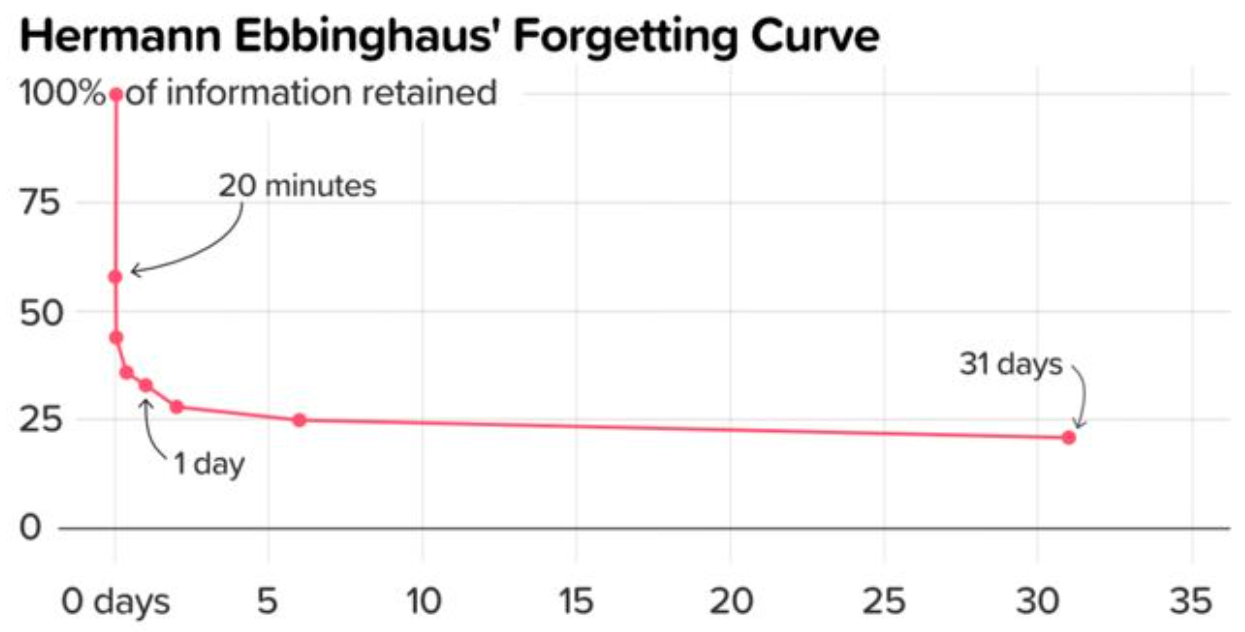
\includegraphics[width=.9\linewidth]{images/ebbinghaus.png}
        \caption{Percentage of retention over time.}
        \label{fig:ebbinghaus}
    \end{subfigure}
    \begin{subfigure}{.49\textwidth}
        \centering
        \captionsetup{width=.8\linewidth}
        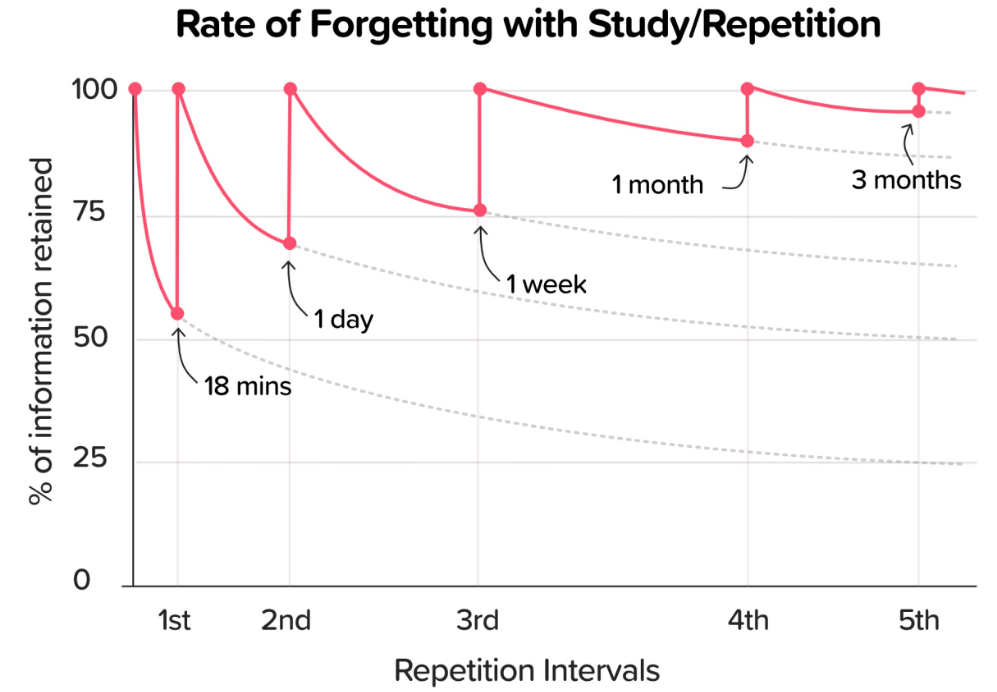
\includegraphics[width=.85\linewidth]{images/ebbinghaus_2.png}
        \caption{Proportion of data retained in function of the repetitions.}
        \label{fig:ebbinghaus_2}
    \end{subfigure}
    \caption{Ebbinghaus forgetting curve.}
    \label{fig:ebbinghaus_1}
\end{figure}

\subsection{Barlett}
Barlett, a critic of Ebbinghaus' approach, thought prior knowledge influences memory, as reconstruction is guided by schemata (a schema is a knowledge structure that organizes memory). He thought that learning is impacted by culture and society.
Bartlett (1932) used multiple repetition of recalled material to study distortions over time. Participants were given a 328 word Native American folk tale ``\textit{The War of the Ghosts} \notet" to read twice and then reproduce 15 minutes later and also hours to months later. He found the total recall declined: what was recalled was shaped by the need to form a coherent understandable story in the context of their own cultural knowledge (schemata-concepts). He considered \textbf{memory an active process of construction}: the memorized content is different from the one that was given, as the process of storing (retrieving) in (from) memory is indeed a construction process, that adds and modifies information.

\osst{People have problems recalling this story, even though it is quite simple from a grammatical point of view. This is because it does not follow the typical traits of stories we are used to.}

\subsection{Gestalt psychology}
\begin{wrapfigure}[12]{r}{0pt}
  \centering
  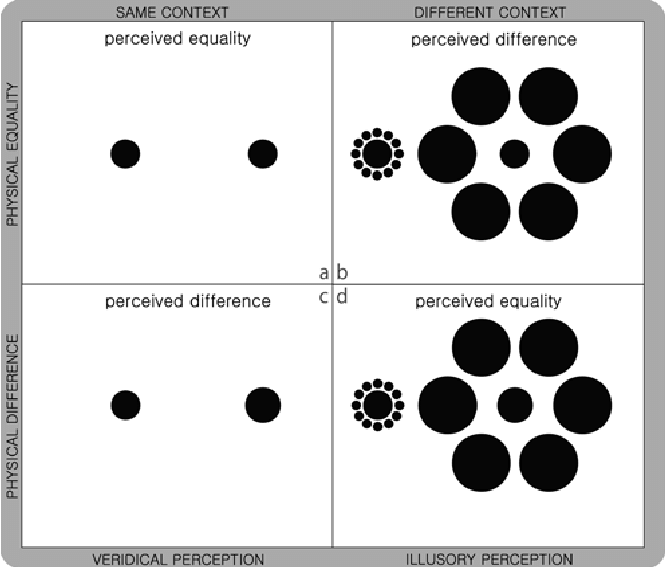
\includegraphics[width=0.3\textwidth]{images/gestalt_2.png}
  \caption{}
  \label{fig:gestalt_2}
\end{wrapfigure}

The Gestalt movement (Kohler, Koffka, Wertheimer) followed an 
\textbf{anti-reductionistic} approach, thinking that a representation cannot be reduced to the representations of its parts (\textit{the whole is different that the sum of its parts}). Yet they did acknowledge the importance of understanding the components of thought.\\

In their view, \textbf{memory is influenced by the configuration of elements and context}, and there is an \textbf{isomorphism of mental representation}: material is represented mentally in the same configuration as it exists in the world. An example of how context impacts perception is provided in Fig.~\ref{fig:gestalt_2}.\\

\details{Gestalt principles: the impact of context}{
\vspace{-0.5cm}
\begin{center}
    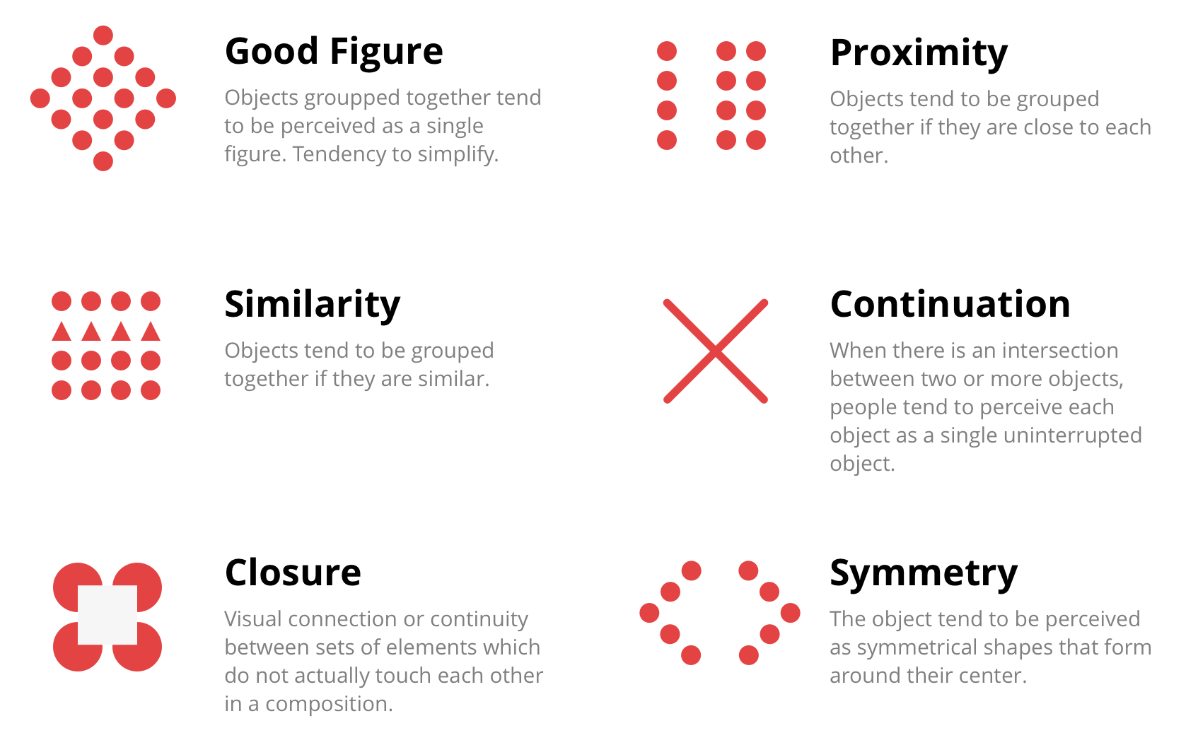
\includegraphics[width=0.6\linewidth]{images/gestalt.png}
\end{center}
}

\subsection{Behaviorism}
Pavlov and Thorndike developed this theory as a response to Gestalt psychology (as this was non quantitative). They thought \textbf{psychology should be the study of observable behavior, not of the structure of mind}. They wanted to quantify behavior; behaviorism is associated with the term \textit{learning} as it is easy to quantify learning. Later behaviorists (like Tolman) used mental explanations and representations (e.g. cognitive maps).\\
From Ebbinghaus's work, they developed a behaviorist approach to the learning of verbal materials (\textbf{verbal learning}: words, sentences, stories): \textbf{memorization is the ``attachment of responses to stimuli"}, while forgetting is the ``loss of response availability".

\subsection{Early neuroscience}
Lashley searched for the brain engram (the physical memory trace). He made rats learn a maze, then he progressively removed larger and larger portions of rats brains from different locations and tested them in the maze to see how memory changed. He found memory was affected more by the amount of brain tissue removed, not the location \notet.

\osst{These conclusions are not valid today, however the question is still important: is memory stored locally or in a distributed/modular way?}

\subsection{Hebb}
Hebb (1949) proposed that cortical organization occurs through ``cell assemblies" and ``phase sequences":
\begin{itemize}
    \item a cell assembly is a set of associated neurons that work together because they are activated together.
    \item Phase sequences incorporate several cell assemblies. They form systems involving multiple interconnected areas of the brain.
\end{itemize}
Repeated stimulation produces structural changes at the synaptic level. The Hebb's rule is ``\textit{What fires together wires together}".

\subsection{The cognitive revolution in psychology}
\begin{wrapfigure}[14]{r}{0pt}
  \centering
  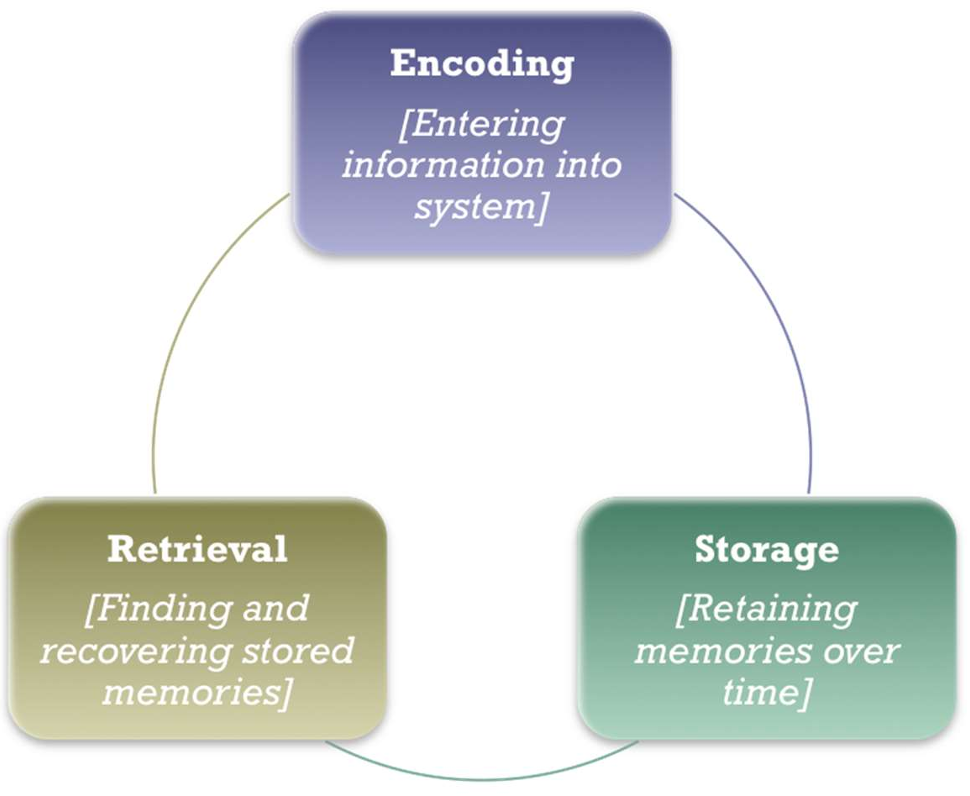
\includegraphics[width=0.4\textwidth]{images/metaphor.png}
  \caption{Like a computer, human memory consists of three interacting components.}
  \label{fig:metaphor}
\end{wrapfigure}
The \textbf{cognitive revolution} consists in the introduction of set of principles that goes against all previous works.
The topic of \textbf{psychology is the study of \textit{thought} by using a quantitative approach}.
Cognitive psychology is the field of psychology associated with the term ``memory", and cognitive psychologists adopt the methodological rigor of the behaviorists.\\

Within cognitive psychology there are three definitions of memory:
\begin{itemize}
    \item The location where memory is stored.
    \item The physical entity that holds the memory (biological representation in brain activity), either \textit{trace} or \textit{engram} (biological storage of a trace)
\end{itemize}

\begin{itemize}
    \item The processes used to acquire (learn), store (encode) or remember (retrieve) information.
\end{itemize}
We can see a parallelism in computers: hardware (brain) vs software (thought processes), and Fig. \ref{fig:metaphor} shows the\textit{ information processing 
metaphor}.
